\documentclass[referee,pdflatex,sn-basic,Numbered]{sn-jnl}
\usepackage{graphicx}
\usepackage{amsmath}
\usepackage{booktabs}
\usepackage{array}
\makeatletter
\newenvironment{landscape}{%
\clearpage
\begingroup
\pdfpagewidth=297mm
\pdfpageheight=210mm
\setlength{\textwidth}{267mm}
\setlength{\textheight}{180mm}
\setlength{\columnwidth}{\textwidth}
\setlength{\linewidth}{\textwidth}
\hsize=\textwidth
\vsize=\textheight
\@colroom=\textheight
}{%
\clearpage
\endgroup
\pdfpagewidth=210mm
\pdfpageheight=297mm
}
\makeatother
\raggedbottom
\emergencystretch=2em

\begin{document}

\title[Self-supervised reproductive life-course phenotyping in the NSFG]{Self-supervised reproductive life-course phenotyping in the National Survey of Family Growth}
\author[1]{\fnm{Feifan} \sur{Lu}}
\email{luff94@163.com}
\equalcont{These authors contributed equally to this work.}
\author[1]{\fnm{Fengshang} \sur{Yan}}
\email{342082145@qq.com}
\equalcont{These authors contributed equally to this work.}
\author[1]{\fnm{Qianqian} \sur{Yang}}
\email{yangqianqian8733@163.com}
\equalcont{These authors contributed equally to this work.}
\author*[1]{\fnm{Jiuqiong} \sur{Yan}}
\email{yanjiuqiong@163.com}
\author*[1]{\fnm{Rui} \sur{Guan}}
\email{cngreen785@163.com}
\affil*[1]{\orgdiv{Department of Obstetrics and Gynecology}, \orgname{Changhai Hospital, Naval Medical University}, \orgaddress{\postcode{200433}, \city{Shanghai}, \country{China}}}

\abstract{
\textbf{Objective:} To develop and evaluate a split-aware self-supervised representation-learning workflow for summarizing heterogeneous reproductive life-course survey records into interpretable respondent phenotypes.

\textbf{Materials and Methods:} We harmonized National Survey of Family Growth (NSFG) female respondent and female pregnancy files from 2011--2013, 2013--2015, 2015--2017, 2017--2019, and 2022--2023. The primary analysis included females aged 15--44 years. Pregnancy files were aggregated to respondent-level histories and linked by CaseID. A leakage-controlled masked tabular self-supervised learning (SSL) encoder was trained on 2011--2017 records, phenotype selection was performed in 2017--2019, and 2022--2023 was reserved for within-NSFG temporal validation rather than validation in a separate health-system dataset. Endpoint-enrichment intervals used a stratified cluster bootstrap based on public-use \texttt{VEST}/\texttt{VECL} design variables.

\textbf{Results:} The harmonized matrix included 26,478 respondents and 598 cross-cycle columns before feature selection. The training/pretraining, development, and temporal-validation splits included 16,176, 5,409, and 4,893 respondents, respectively. The primary encoder used 48 endpoint-excluded features and generated 48-dimensional respondent embeddings. Development-cycle clustering selected three phenotypes (silhouette 0.606; Davies--Bouldin 0.701; bootstrap adjusted Rand index 0.914). In 2022--2023, P0 represented younger low-pregnancy-exposure respondents, P1 represented the main pregnancy-exposed phenotype, and P2 was a small high-burden pregnancy-history phenotype. Within respondents with at least one pregnancy record, P2 showed the highest enrichment for adverse pregnancy-history proxy (prevalence ratio [PR] 2.16; 95\% CI 1.60--2.85; 48/229 events) and mistimed or unwanted pregnancy history (PR 1.17; 95\% CI 1.09--1.25; 181/229 events). Full-cohort estimates were larger, consistent with partial mechanical enrichment from pregnancy exposure. SSL embeddings had higher AUPRC than raw 48 encoder inputs in 5/5 full-cohort endpoints and 2/2 ever-pregnant pregnancy-history endpoints. Adjusted models supported P2 enrichment for adverse pregnancy-history proxy (adjusted OR 2.05, 95\% CI 1.20--3.57) and P1 enrichment for contraceptive vulnerability (adjusted OR 1.84, 95\% CI 1.39--2.41), whereas fecundity limitation/infertility in P2 was not robust after adjustment.

\textbf{Discussion:} The workflow provides an informatics framework for representation learning, phenotype discovery, leakage auditing, and temporal stress testing in complex reproductive-health survey data. Pregnancy-history enrichment required interpretation against age/parity and ever-pregnant baselines.

\textbf{Conclusion:} Masked tabular SSL can summarize NSFG respondent and pregnancy records into interpretable reproductive life-course profiles and reproducible endpoint-enrichment summaries. The study supports survey representation learning and phenotype discovery, not clinical diagnosis, individual treatment guidance, or causal inference.
}

\keywords{National Survey of Family Growth, reproductive health, self-supervised learning, life-course phenotyping, contraception, fertility}

\maketitle

\section*{Lay Summary}

Large reproductive-health surveys contain information about contraception, pregnancy histories, fertility care, relationships, insurance, and socioeconomic conditions, but these domains are often analyzed one at a time. We developed a self-supervised learning workflow that summarizes many survey variables into respondent-level representations and then groups respondents into interpretable reproductive life-course profiles. The workflow was trained on earlier National Survey of Family Growth cycles and evaluated in the 2022--2023 cycle. The learned profiles highlighted groups with different reproductive histories and different concentrations of survey-defined endpoints such as contraceptive vulnerability, fertility-service or pregnancy-loss help, mistimed or unwanted pregnancy history, and adverse pregnancy-history proxies. The study is intended as a reproducible informatics approach for population-level survey phenotyping and hypothesis generation. It should not be used as a clinical diagnosis, individual risk calculator, treatment recommendation tool, or causal analysis.

\section{Background and Significance}

Reproductive health is rarely determined by a single exposure. Contraceptive use, pregnancy timing, pregnancy outcomes, partnership history, fertility services, fecundity limitation or infertility, health insurance, and socioeconomic conditions can co-occur across the reproductive life course. National studies have separately characterized unintended pregnancy, contraceptive failure or non-use, infertility, and fertility-service use using NSFG and related reproductive-health surveillance data \cite{finer_zolna_unintended,contraceptive_failure,infertility_impaired,infertility_service,contraceptive_nonuse}. Analyses that isolate one domain are valuable for surveillance, but they may understate heterogeneity among respondents whose reproductive histories and social conditions jointly shape reproductive-health needs.

The National Survey of Family Growth (NSFG) is a nationally representative United States survey that gathers information on fertility, contraception, pregnancy and births, marriage and cohabitation, infertility, and reproductive health. The public-use female respondent and female pregnancy files can be joined by CaseID, enabling respondent-level summaries of pregnancy histories while preserving a reproducible public-data workflow \cite{cdc_nsfg_puf,cdc_nsfg_combined}. Recent NCHS reports using the 2022--2023 NSFG have described current contraceptive status, fertility-service use, and birth expectations \cite{cdc_db539,cdc_db542,cdc_db560}. These reports provide essential national estimates, but they are not designed to learn multivariable reproductive life-course phenotypes across respondent and pregnancy records.

Self-supervised learning for tabular data offers a practical approach for learning representations from sparse, heterogeneous survey variables without using a single supervised label during representation training. Prior tabular SSL and transformer methods, including VIME, TabTransformer, SAINT, and SCARF, support the use of masking, contextual feature embeddings, and corruption-based pretraining for tabular representation learning \cite{vime,tabtransformer,saint,scarf}. Drawing on these ideas, we implemented a compact masked-reconstruction encoder for the public-use NSFG setting with explicit temporal splitting and endpoint leakage control; contrastive, row-attention, and large-scale foundation-model variants were not implemented.

\section{Objective}

This study aimed to construct a respondent-level reproductive life-course matrix from NSFG files, train a masked tabular SSL encoder using earlier cycles, identify interpretable reproductive phenotypes in a development cycle, and evaluate phenotype-associated enrichment of prespecified reproductive-health endpoints in the temporally held-out 2022--2023 release.

\section{Methods}

\subsection{Data sources and study population}

We used public-use NSFG female respondent and female pregnancy files from 2011--2013, 2013--2015, 2015--2017, 2017--2019, and 2022--2023. Fixed-width 2011--2019 files were parsed with official CDC Stata dictionaries. The 2022--2023 public-use CSV files and user guide were obtained from the CDC/NCHS NSFG public-use data page. The primary analysis was restricted to females aged 15--44 years to preserve comparability between 2011--2019 and 2022--2023 public-use releases. The 2022--2023 NSFG release used a redesigned continuous, multimode protocol with an online component; therefore, the held-out cycle should be interpreted as a within-NSFG temporal and survey-mode stress test rather than a pure calendar-time validation. Cohort characteristics by temporal split are shown in Table 1.

\begin{table}[tbp]
\centering
\caption{Cohort characteristics by temporal analysis split. Weighted estimates use public-use NSFG analysis weights; model training did not use survey weights as input features. Values for age and parity are weighted mean (SD). Endpoint percentages use the full analytic respondent denominator and therefore represent survey-level endpoint proxies rather than pregnancy-record-only rates.}
\label{tab:cohort}
\footnotesize
\setlength{\tabcolsep}{4pt}
\begin{tabular*}{\textwidth}{@{\extracolsep{\fill}}>{\raggedright\arraybackslash}p{0.34\textwidth}rrr@{}}
\toprule
Characteristic & Training/pretraining & Development & Temporal validation \\
\midrule
Respondents, n & 16,176 & 5,409 & 4,893 \\
Age, years, mean (SD) & 29.6 (8.5) & 29.6 (8.4) & 29.6 (8.6) \\
Parity, mean (SD) & 1.19 (1.38) & 1.09 (1.35) & 0.99 (1.39) \\
Any pregnancy record, \% & 61.1 & 56.4 & 50.0 \\
Contraceptive vulnerability, \% & 7.2 & 7.2 & 7.8 \\
Fertility/loss help, \% & 11.5 & 10.4 & 11.1 \\
Mistimed/unwanted pregnancy history, \% & 47.8 & 44.7 & 34.2 \\
Adverse pregnancy-history proxy, \% & 9.9 & 8.5 & 5.4 \\
Fecundity limitation/infertility, \% & 28.0 & 28.7 & 28.1 \\
\bottomrule
\end{tabular*}
\end{table}


\subsection{Temporal split and leakage control}

The 2011--2013, 2013--2015, and 2015--2017 cycles were used for SSL pretraining. The 2017--2019 cycle was used for phenotype model selection and development-cycle diagnostics. The 2022--2023 cycle was reserved for within-NSFG temporal validation, and its endpoint labels were used only for final evaluation. This design evaluates temporal transport within a public-use survey series, not validation in a separate health-system cohort or registry. Survey weights were retained for descriptive prevalence and phenotype profiles, but were not used as model inputs because the encoder was intended to learn a reusable respondent-level representation from harmonized public-use variables rather than estimate design-weighted national parameters during optimization. For the primary encoder, variables directly defining the validation endpoints were excluded before feature selection to reduce endpoint leakage. Figure 1 summarizes the temporal split, leakage-controlled matrix construction, masked tabular SSL encoder, phenotype discovery, and validation workflow.

\begin{figure}[htbp]
\centering
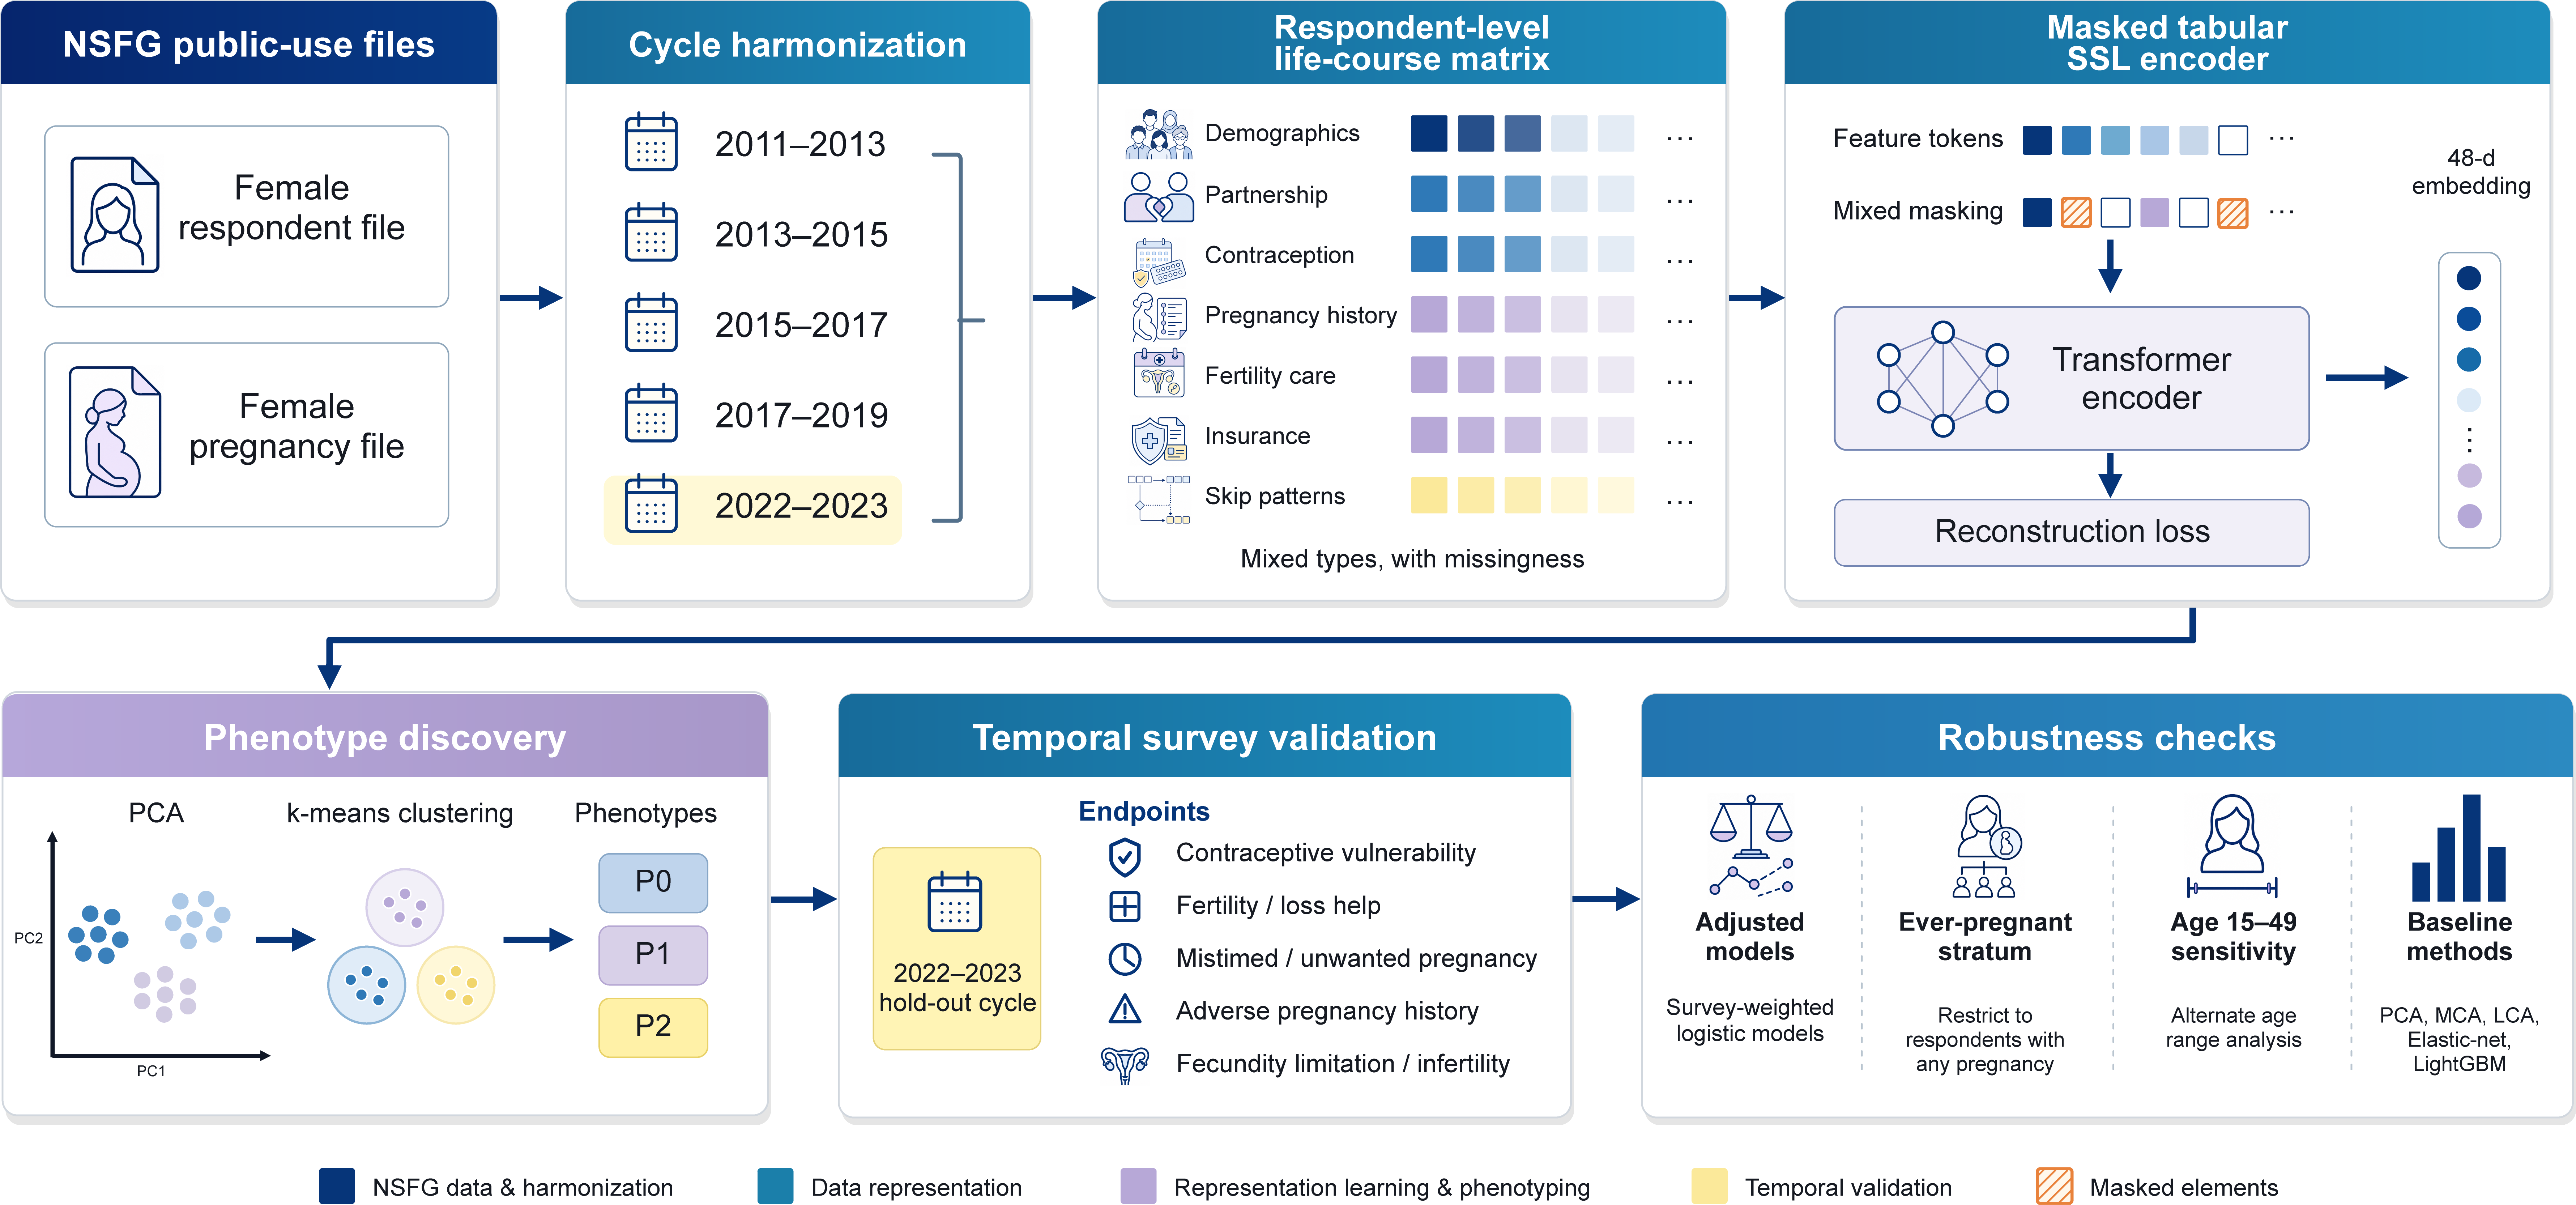
\includegraphics[width=\textwidth]{figures/FIG1.png}
\caption{Study design and leakage-controlled analysis workflow. Public-use NSFG female respondent and female pregnancy files were harmonized across cycles. Earlier cycles were used for masked SSL pretraining, 2017--2019 for phenotype selection, and 2022--2023 for within-NSFG temporal and survey-mode stress testing. Endpoint-direct variables were excluded from the primary encoder input.}
\label{fig:workflow}
\end{figure}

\subsection{Respondent-level life-course matrix}

Female pregnancy records were aggregated to respondent level using pregnancy counts, live-birth and pregnancy-outcome counts, pregnancy-intention summaries, low-birthweight or stillbirth proxies, and prenatal-care or smoking indicators where public-use variables were available. These summaries were joined to female respondent variables by CaseID. Candidate input domains included demographics and social factors, partnership and marriage, reproductive timing, sexual and contraceptive history, pregnancy-history summaries, fertility and reproductive-health indicators, insurance and poverty, and missingness or skip-pattern indicators. Table 2 lists the primary input domains, endpoint definitions, and leakage-control rules used before SSL fitting.

\begin{table}[tbp]
\centering
\caption{Input feature set and validation endpoint definitions. Direct endpoint-defining variables were excluded from the primary encoder input before SSL fitting. The fecundity-limitation endpoint excludes contraceptive sterilization from the FECUND recode.}
\label{tab:endpoints}
\scriptsize
\setlength{\tabcolsep}{4pt}
\begin{tabular*}{\textwidth}{@{\extracolsep{\fill}}>{\raggedright\arraybackslash}p{0.20\textwidth}>{\raggedright\arraybackslash}p{0.42\textwidth}c>{\raggedright\arraybackslash}p{0.22\textwidth}@{}}
\toprule
Domain or endpoint & Operational definition & Role & Leakage-control rule \\
\midrule
Primary SSL input features & Endpoint-direct variables excluded; top nonconstant features selected by train-set completeness and variance. & 48 & Direct endpoint regex excluded before encoder fitting. \\
Contraceptive vulnerability & CONSTAT1 code 42; denominator is the NSFG analytic female respondent population, interpreted as a current vulnerability proxy rather than an incident pregnancy outcome & Endpt. & Direct endpoint-variable regex excluded; full regex retained in source-data table. \\
Fertility or loss help & HLPPRG code 1 or HLPMC code 1, indicating ever receiving medical help to become pregnant or to prevent miscarriage & Endpt. & Direct endpoint-variable regex excluded; full regex retained in source-data table. \\
Mistimed or unwanted pregnancy history & Among respondents with pregnancy records, any NEWWANTR code 3/4/6, WANTRESP code 3/5, WANTPART code 3/5, TIMINGOK code 3, or WANTBOLD code 5 & Endpt. & Direct endpoint-variable regex excluded; full regex retained in source-data table. \\
Adverse pregnancy-history proxy & Among respondents with pregnancy records, any public-use low-birthweight live birth indicator (LBW1 code 1) or stillbirth outcome (OUTCOME code 3) & Endpt. & Direct endpoint-variable regex excluded; full regex retained in source-data table. \\
Fecundity limitation or infertility & FECUND code 2-5 or INFERT code 1-2, using public-use NSFG fecundity or infertility recodes and excluding FECUND code 1 contraceptive sterilization & Endpt. & Direct endpoint-variable regex excluded; full regex retained in source-data table. \\
\bottomrule
\end{tabular*}
\end{table}


\subsection{Masked tabular SSL encoder}

The primary model used a masked tabular SSL encoder implemented for numeric-coded public-use survey variables. Feature values were median-imputed and standardized using training-cycle parameters, and missingness indicators were supplied as token inputs. During training, 15\% of observed values were masked and the model minimized masked reconstruction mean squared error. The compact encoder used 1 transformer encoder layer, hidden dimension 32, 4 attention heads, dropout 0.10, batch size 1024, AdamW optimization with learning rate 0.001, and 30 training epochs. The final analysis artifacts used 48 endpoint-excluded input features and 48-dimensional respondent embeddings. This model was designed as a compact public-survey representation learner, not as a large foundation model.

All preprocessing and representation steps were fitted within their designated temporal splits. Training-cycle records were used to estimate imputation medians, standardization parameters, feature-completeness and variance screens, SSL encoder parameters, and principal-component loadings. Development-cycle embeddings were used to select k and fix k-means centroids. The 2022--2023 endpoint labels were not used for feature screening, imputation, scaling, PCA fitting, centroid fitting, SSL model selection, or phenotype naming. Endpoint-defining variable patterns and the primary encoder feature-audit file are provided in Table 2 and the source-data directory.

\subsection{Phenotype discovery and validation}

Respondent embeddings were projected to principal components fitted on training-cycle embeddings. The number of phenotypes was selected in 2017--2019 by comparing k=2--8 using silhouette score, Davies--Bouldin index, minimum cluster proportion, and 60 bootstrap adjusted Rand index (ARI) resamples. Development-cycle centroids were then fixed, and 2022--2023 respondents were assigned to the nearest centroid. Phenotype descriptions were based on survey-weighted profile characteristics, not on outcome enrichment alone.

Five validation endpoints were prespecified: contraceptive vulnerability, fertility-service or pregnancy-loss help, mistimed or unwanted pregnancy history, adverse pregnancy-history proxy, and fecundity limitation/infertility. The contraceptive-vulnerability endpoint was defined from the NSFG current contraceptive-status recode and interpreted as a current contraceptive at-risk status proxy within the analytic respondent population rather than an incident pregnancy outcome. The fecundity endpoint used \texttt{FECUND} codes for noncontraceptive surgical sterility, nonsurgical sterility, subfecundity, or long interval plus \texttt{INFERT} codes indicating infertility, and excluded contraceptive sterilization. Pregnancy-history endpoints used respondent-level pregnancy-file summaries and were interpreted as self-reported survey-history proxies rather than clinically adjudicated pregnancy outcomes. Because pregnancy exposure itself can mechanically affect pregnancy-history endpoint rates, the ever-pregnant stratum restricted to respondents with at least one pregnancy record in the public-use pregnancy file was used as the primary interpretive enrichment analysis for the two pregnancy-history endpoints; full-cohort estimates were retained as supporting exposure-structured summaries. Endpoint enrichment was summarized using survey-weighted one-vs-rest prevalence ratios and risk differences, following complex-survey analysis principles for descriptive population summaries \cite{lumley_survey}. In these one-vs-rest contrasts, each phenotype is compared with its complement, so estimates for the majority phenotype can be pulled toward the null by construction. AUPRC enrichment was defined as AUPRC divided by the endpoint baseline prevalence. Uncertainty intervals for endpoint enrichment were estimated with a stratified cluster percentile bootstrap using public-use \texttt{VEST} strata and \texttt{VECL} cluster variables, retaining the public-use respondent weights in each resample; the 2022--2023 primary bootstrap used 20 strata, 80 stratum-cluster pairs, and 2000 resamples. Intervals were treated as descriptive because no multiplicity adjustment was applied across endpoints, phenotypes, and robustness families.

Secondary supervised endpoint-enrichment models compared simple reproductive-exposure variables (age, parity, and ever-pregnant status), raw primary encoder inputs, SSL embeddings, raw inputs plus SSL embeddings, phenotype-only inputs, and SSL-plus-phenotype inputs using L2-regularized logistic regression. Raw-feature and simple-exposure baselines were included because neural-network representations do not automatically outperform strong non-deep or direct tabular baselines \cite{tabular_tree}. Models were trained on 2011--2019 records, features were standardized within the training data, class weights were balanced, and 2022--2023 labels were used only for final evaluation. AUPRC, AUPRC enrichment over baseline prevalence, and AUROC were reported as unweighted model-performance summaries, whereas phenotype prevalence profiles and endpoint-enrichment estimates used survey weights. These supervised summaries were used to assess representation utility against raw-feature and trivial reproductive-exposure baselines; they were not interpreted as bedside diagnostic models, individual prognostic models, treatment-decision tools, or calibrated absolute-risk tools.

\subsection{Robustness and sensitivity analyses}

Seven robustness analyses were added after the primary workflow was fixed. First, because the 2022--2023 NSFG release includes females aged 15--49 years whereas earlier public-use cycles were restricted to ages 15--44 years, we transferred the trained endpoint-excluded encoder to the full 2022--2023 age range and compared endpoint enrichment in ages 15--44 versus 15--49 years without refitting the encoder, PCA, or development-cycle centroids. Second, we fitted survey-weighted one-vs-rest logistic enrichment models for each endpoint and phenotype, adjusting for age, race/ethnicity, education, poverty, insurance, and parity; confidence intervals used a stratified cluster bootstrap with \texttt{VEST}/\texttt{VECL}. These adjusted models were descriptive enrichment checks rather than causal models. Third, we compared SSL phenotyping with raw matrix PCA plus k-means, MCA-style one-hot SVD plus k-means, and selected-variable Bernoulli latent class analysis, interpreting stability and cluster degeneracy alongside endpoint enrichment. Fourth, we trained a full-domain SSL sensitivity encoder that did not exclude endpoint-direct variables and compared enrichment with the primary endpoint-excluded encoder. Fifth, subgroup robustness was summarized across age group, race/ethnicity, poverty, insurance, and parity strata. Sixth, we constructed simple age-by-parity and age-by-ever-pregnant strata to test whether pregnancy-history endpoint enrichment was recoverable from trivial reproductive-exposure groupings. Seventh, we performed a fixed-k encoder initialization sensitivity analysis by comparing the primary seed with one complete 30-epoch alternative seed while keeping the development-selected k=3 structure; this was treated as a sensitivity check rather than a repeated model-selection experiment.

Reporting was guided by STROBE for observational studies and by TRIPOD+AI items where they were relevant to transparent reporting of machine-learning model development and evaluation \cite{strobe,tripod_ai}. The present study is not a clinical prediction-model development study, so TRIPOD+AI was used as a reporting and transparency reference rather than as a claim that the workflow produces a deployable clinical prediction model.

\section{Results}

\subsection{Cohort and harmonized matrix}

The harmonized analysis included 26,478 respondents across five public-use cycles. Table 1 summarizes cohort characteristics by temporal split. The temporal-validation cohort included 4,893 respondents from 2022--2023. Female pregnancy records were joined to respondent records by CaseID, and Figure 2A reports the share of respondents with at least one pregnancy record rather than a file-linkage success or failure rate. The word ``linkage'' in the display refers to pregnancy-record history coverage after CaseID-based file joining, not to failed linkage among eligible respondent records. The harmonized matrix contained 598 columns before primary feature selection. Figure 2 shows cohort magnitude, pregnancy-record history coverage, input domains, missingness, feature-selection flow, and endpoint prevalence.

\begin{figure}[htbp]
\centering
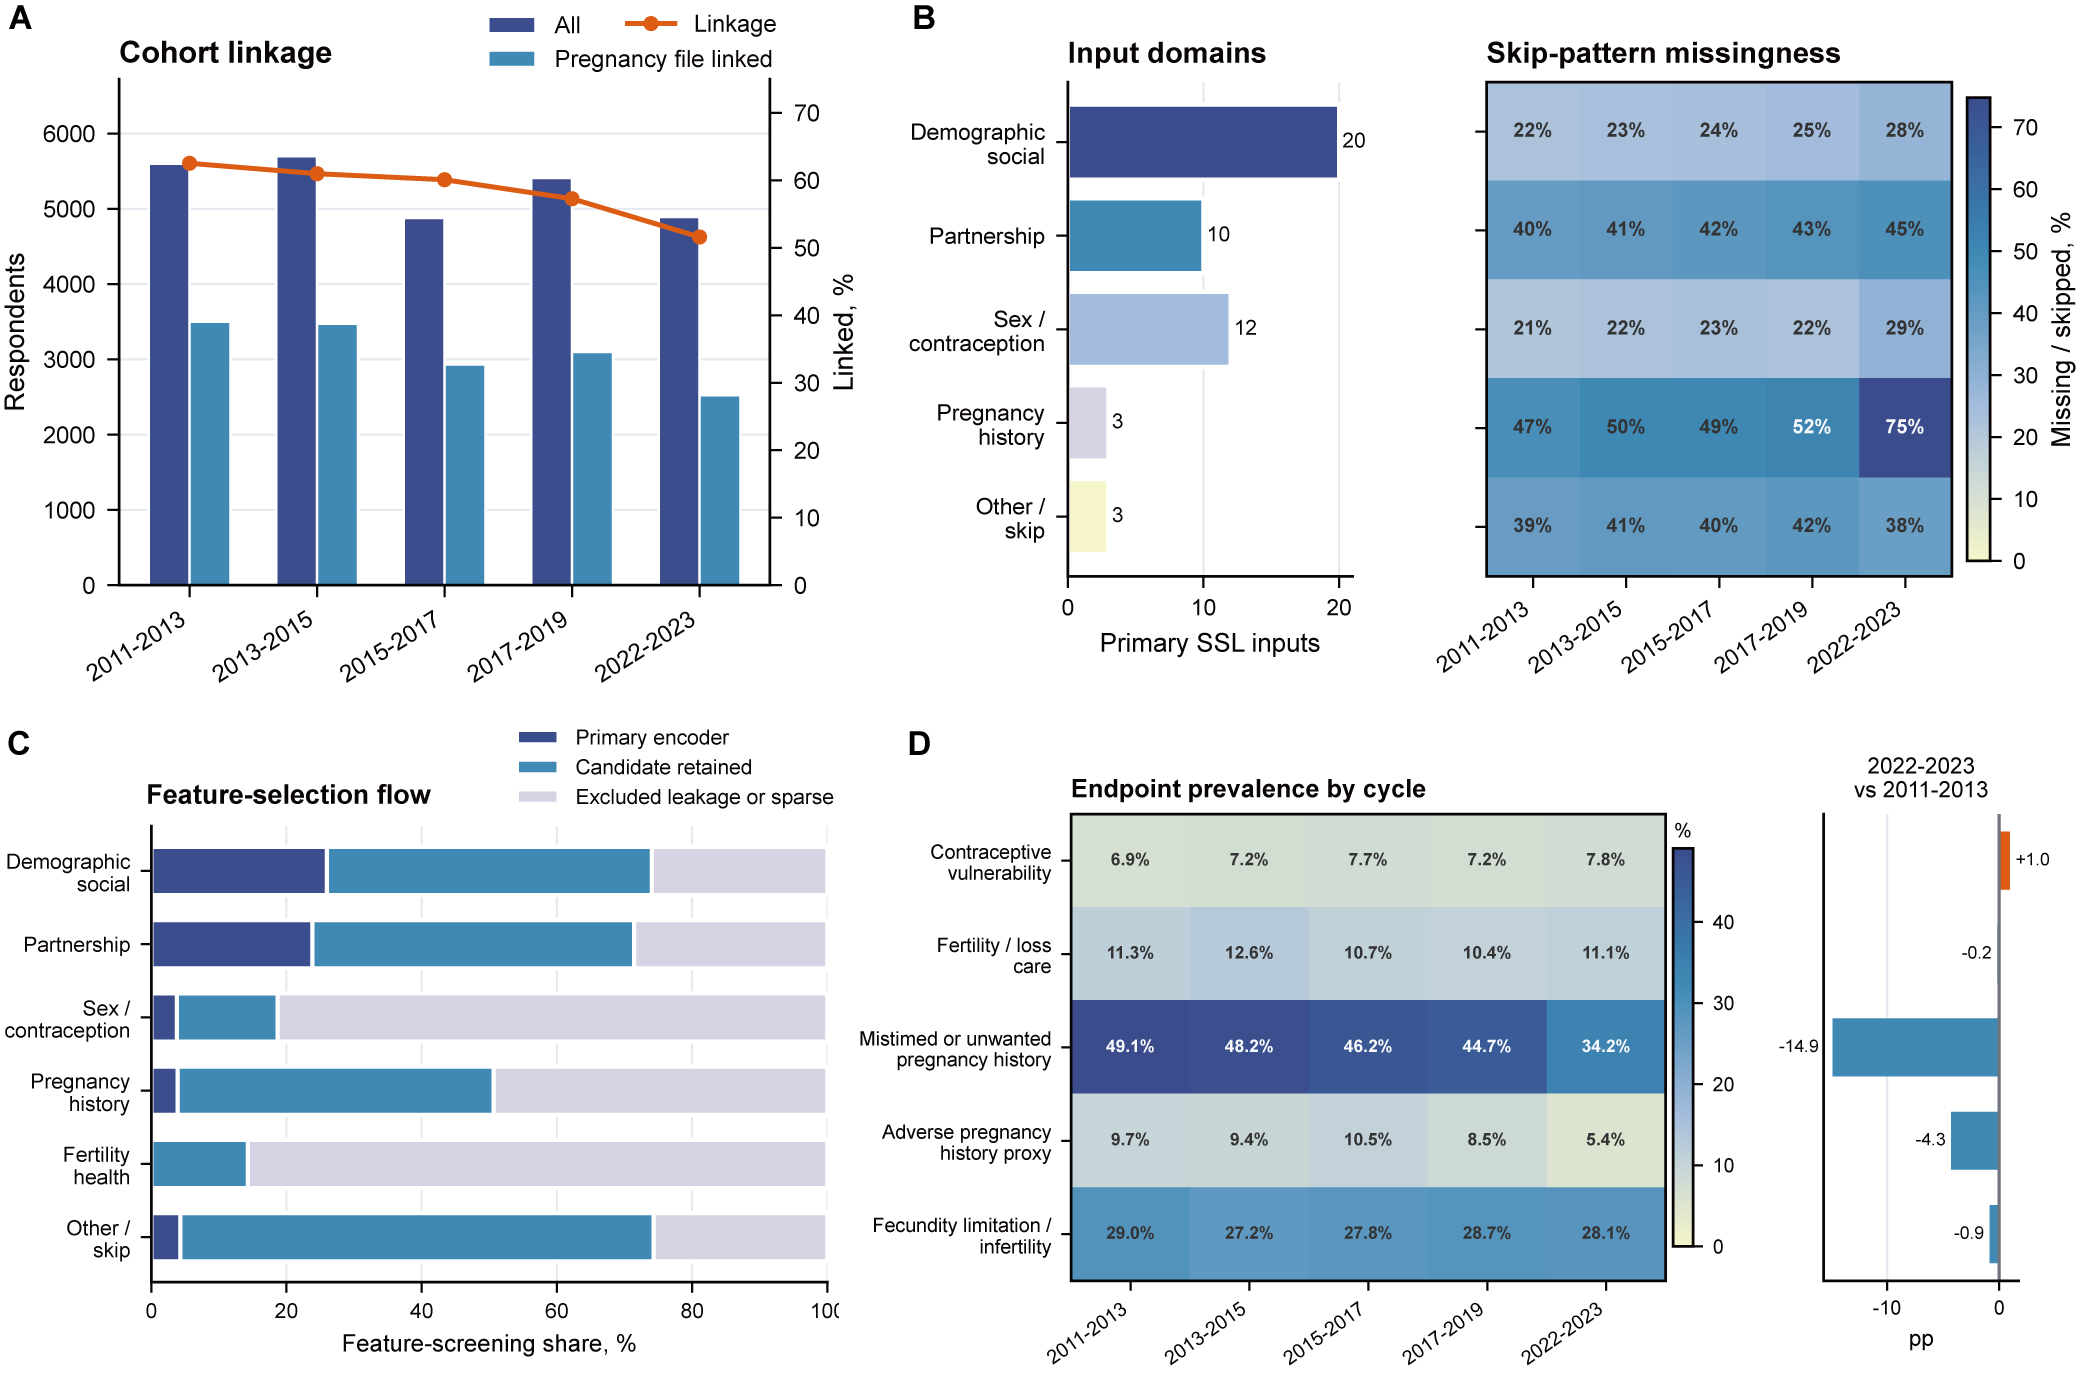
\includegraphics[width=\textwidth]{figures/FIG2.png}
\caption{Harmonized cohort structure, leakage-controlled inputs, feature selection, and endpoint prevalence. (A) Female respondent counts and pregnancy-record history coverage, defined as the number and percentage of respondents with at least one record in the public-use pregnancy file after CaseID-based joining; this is not a pregnancy-file linkage-failure rate. (B) Primary SSL input-domain counts and skip-pattern missingness by cycle. (C) Feature-selection flow separating primary encoder inputs, retained candidate features, and excluded or sparse variables. (D) Weighted endpoint prevalence across cycles with temporal-test change relative to 2011--2013.}
\label{fig:matrix}
\end{figure}

\subsection{SSL phenotype discovery}

The embedding, phenotype sizes, profile drivers, and k-selection evidence are shown in Figure 3; the numerical cluster-selection metrics are given in Supplementary Table 1, and the SSL training diagnostics are shown in Supplementary Figure S5. The masked reconstruction loss declined across 30 SSL training epochs, supporting optimization of the compact encoder while remaining a training diagnostic rather than an outcome-validation metric. In the development cycle, k=3 had the highest silhouette score (0.606) and high bootstrap ARI (0.914) among candidate cluster counts. The k=3 solution was retained over the more balanced k=2 alternative because it isolated an interpretable high-burden pregnancy-history profile while preserving high bootstrap stability. The smallest development-cycle cluster comprised 4.6\% of respondents, below the preferred 5\% threshold; therefore, k=3 was treated as a development-selected, bootstrap-stable, small-cluster solution rather than evidence of a universal reproductive taxonomy.

\begin{figure}[htbp]
\centering
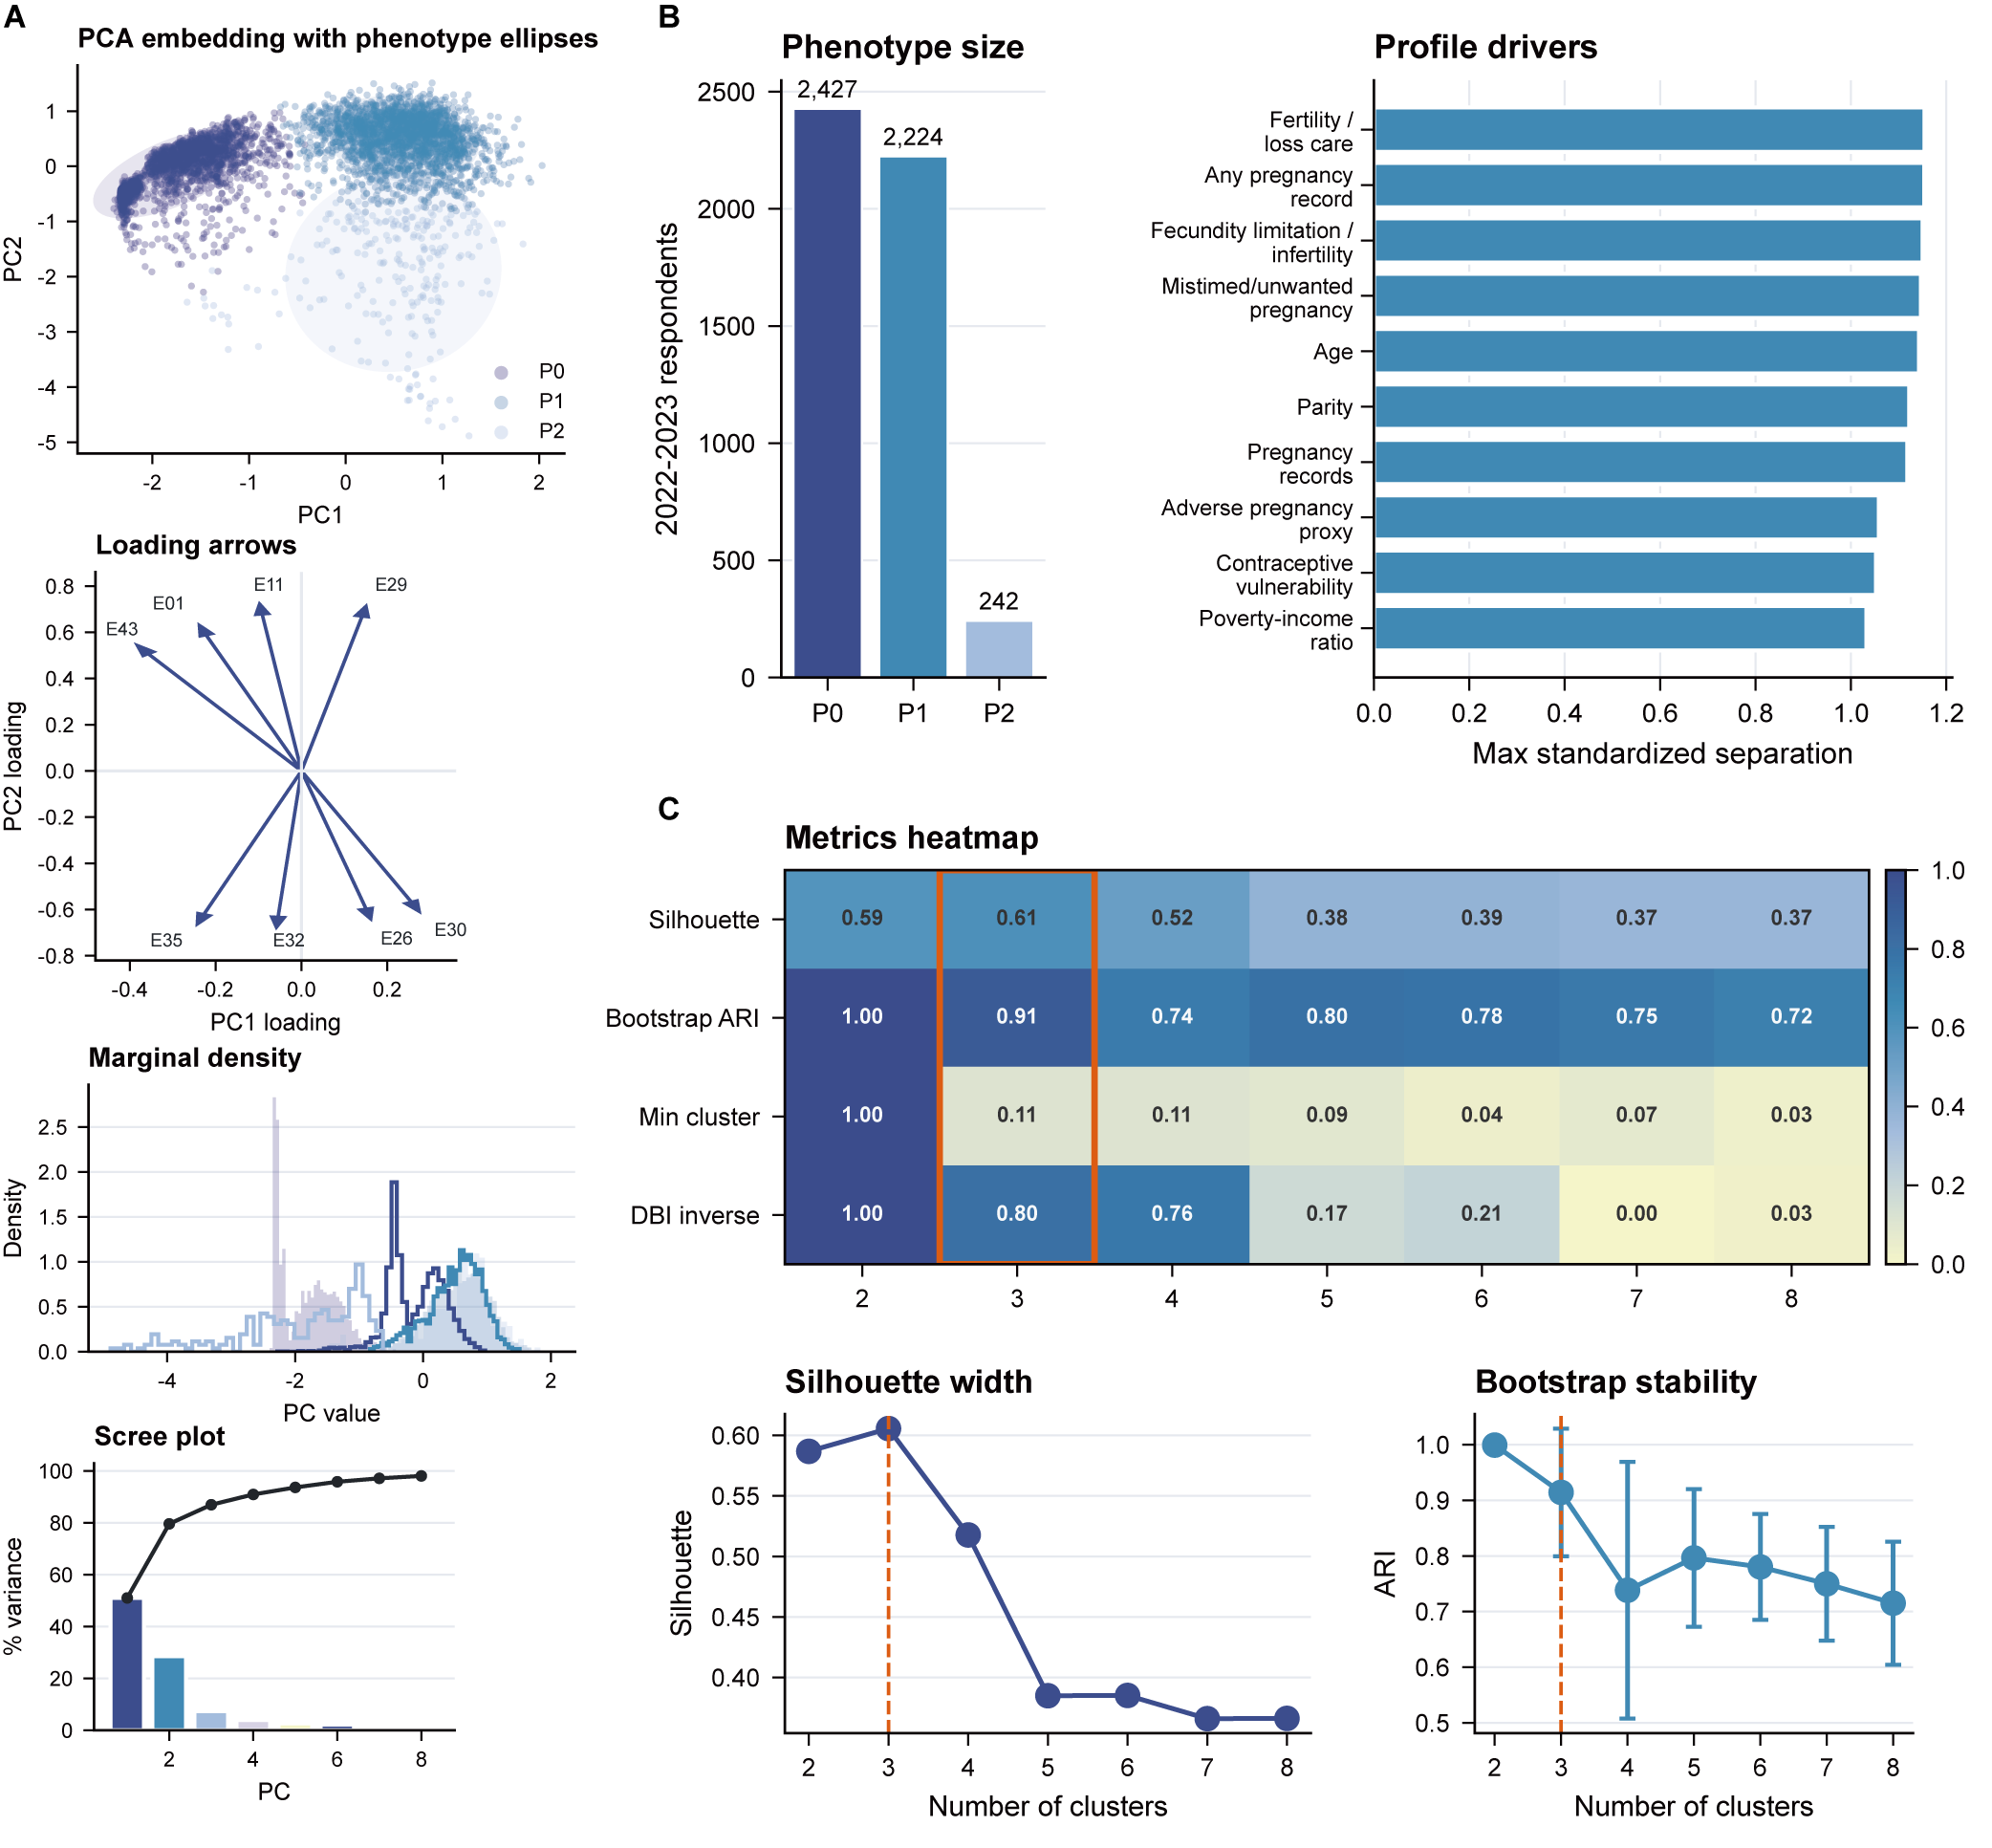
\includegraphics[width=0.95\textwidth]{figures/FIG3.png}
\caption{SSL embedding and phenotype discovery. (A) PCA visualization of 2022--2023 SSL embeddings colored by transferred phenotype, with phenotype ellipses, marginal PC density, leading embedding loadings, and a scree summary. (B) Phenotype size and leading profile drivers. (C) Development-cycle k-selection evidence, including the multi-metric heatmap, silhouette width, and bootstrap adjusted Rand index across candidate cluster numbers.}
\label{fig:phenotypes}
\end{figure}

\subsection{Temporal-validation phenotype profiles}

The survey-weighted phenotype profile patterns are displayed in Figure 4. Table 3 provides the corresponding weighted profile estimates.

In 2022--2023, P0 represented younger low-pregnancy-exposure respondents, with weighted mean age 24.8 years, parity 0.04, and 3.2\% having at least one pregnancy record. P1 represented the main pregnancy-exposed phenotype, with weighted mean age 34.4 years, parity 1.94, 100.0\% having at least one pregnancy record, and the highest contraceptive vulnerability prevalence (10.4\%). P2 was a small high-burden pregnancy-history phenotype, with weighted mean age 36.2 years, parity 2.55, 95.4\% having at least one pregnancy record, adverse pregnancy-history proxy prevalence 22.2\%, mistimed or unwanted pregnancy-history prevalence 76.4\%, and fecundity limitation/infertility prevalence 41.0\%.

\begin{table}[tbp]
\centering
\caption{Survey-weighted temporal-validation phenotype profiles in 2022--2023. Phenotype labels were assigned from development-cycle centroids and named descriptively from profile characteristics, not from outcome status alone.}
\label{tab:phenotype_profiles}
\small
\setlength{\tabcolsep}{6pt}
\begin{tabular*}{\textwidth}{@{\extracolsep{\fill}}>{\raggedright\arraybackslash}p{0.56\textwidth}rrr@{}}
\toprule
Profile characteristic & P0 & P1 & P2 \\
\midrule
Age, years & 24.78 & 34.41 & 36.16 \\
Parity & 0.04 & 1.94 & 2.55 \\
Pregnancy records & 0.05 & 2.61 & 3.50 \\
Any pregnancy record, \% & 3.2 & 100.0 & 95.4 \\
Poverty-income ratio & 340.29 & 278.99 & 229.24 \\
Contraceptive vulnerability, \% & 5.6 & 10.4 & 7.6 \\
Fertility or loss help, \% & 4.3 & 18.2 & 18.6 \\
Mistimed/unwanted pregnancy, \% & 2.3 & 67.0 & 76.4 \\
Adverse pregnancy-history proxy, \% & 0.5 & 9.2 & 22.2 \\
Fecundity limitation/infertility, \% & 17.8 & 38.8 & 41.0 \\
\bottomrule
\end{tabular*}
\end{table}


\begin{figure}[htbp]
\centering
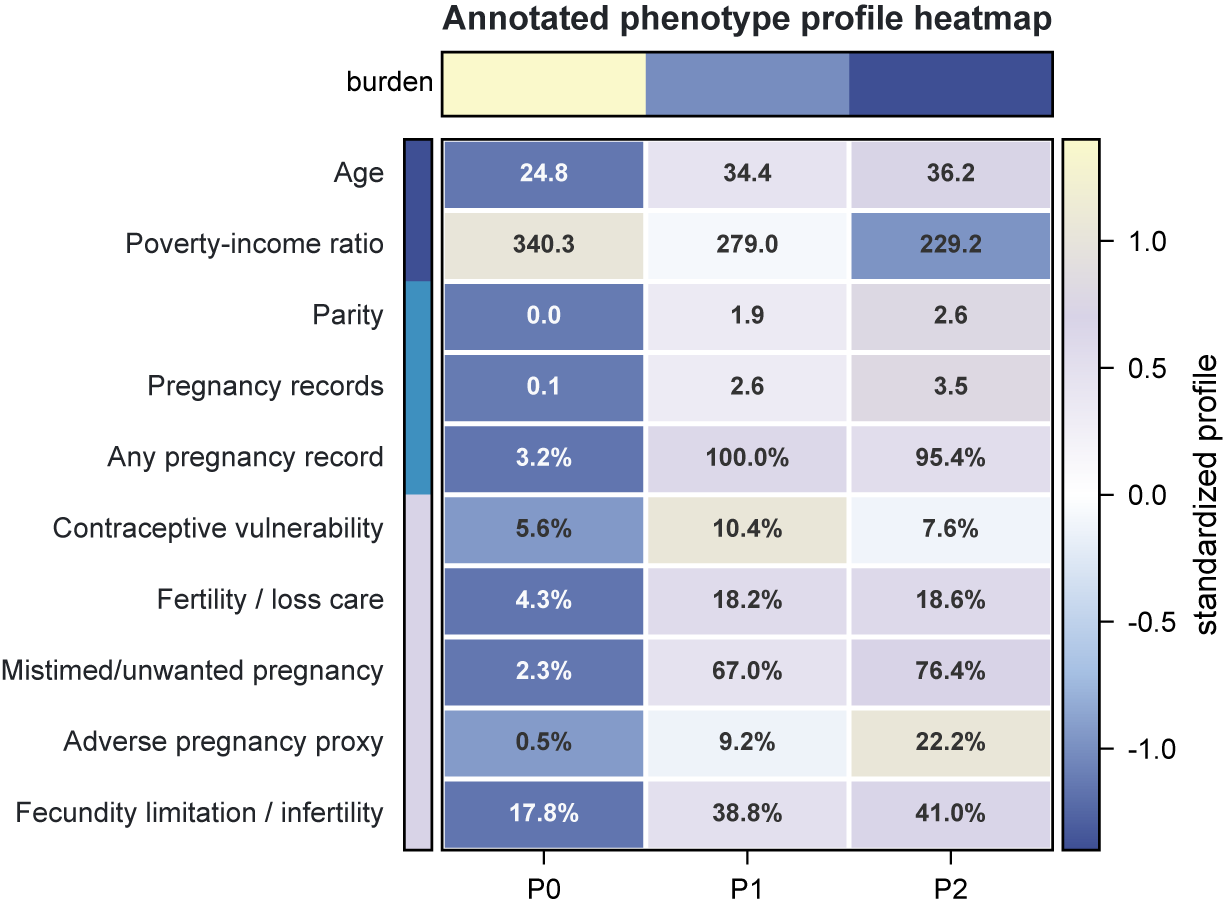
\includegraphics[width=0.92\textwidth]{figures/FIG4.png}
\caption{Survey-weighted phenotype profiles in 2022--2023. Heatmap cells show standardized deviations across phenotypes for selected reproductive life-course descriptors and endpoint-related characteristics; cell labels show weighted raw means or prevalences. The top annotation bar summarizes a relative profile-burden score derived from pregnancy-record count and adverse pregnancy-history proxy; the left annotation bar groups rows into sociodemographic, pregnancy-history, and endpoint-related descriptor families.}
\label{fig:profiles}
\end{figure}

\subsection{Endpoint enrichment and secondary supervised validation}

Bootstrap source estimates for endpoint enrichment and uncertainty intervals are provided in Supplementary Table 2. Pregnancy-history endpoint enrichment was interpreted primarily within respondents with at least one pregnancy record in the public-use pregnancy file, because full-cohort contrasts are partly driven by the low-pregnancy-exposure P0 phenotype. In this ever-pregnant stratum, P2 was enriched for adverse pregnancy-history proxy (48/229 events; PR 2.16, 95\% CI 1.60--2.85) and mistimed or unwanted pregnancy history (181/229 events; PR 1.17, 95\% CI 1.09--1.25). Full-cohort estimates were larger for the same endpoints (adverse pregnancy-history proxy PR 4.13; 95\% CI 2.98--5.46; mistimed or unwanted pregnancy history PR 2.23; 95\% CI 2.06--2.43), consistent with mechanical enrichment from pregnancy exposure and therefore treated as supporting rather than primary evidence.

For endpoints not structurally restricted to pregnancy records, full-cohort enrichment was summarized in the 2022--2023 analytic cohort. P2 was enriched for fertility-service or pregnancy-loss help (44/242 events; PR 1.67; 95\% CI 1.19--2.19) and fecundity limitation/infertility (94/242 events; PR 1.46; 95\% CI 1.22--1.69). P1 showed the highest enrichment for contraceptive vulnerability, interpreted here as a current contraceptive at-risk status proxy (238/2224 events; PR 1.33; 95\% CI 1.22--1.44), consistent with its larger pregnancy-exposed profile and higher current contraceptive vulnerability prevalence.

Secondary supervised summaries showed that SSL embeddings carried endpoint-enrichment information beyond raw-feature and simple reproductive-exposure baselines in this temporal split. SSL embeddings had higher AUPRC than the raw 48 primary encoder inputs for 5/5 full-cohort endpoints and 2/2 ever-pregnant pregnancy-history endpoints. For example, contraceptive-vulnerability AUPRC increased from 0.124 with raw 48 inputs to 0.472 with SSL embeddings, and ever-pregnant adverse pregnancy-history proxy AUPRC increased from 0.173 to 0.190. Because indirect survey proxies can still exist after direct endpoint-variable exclusion, these supervised differences were interpreted as representation-utility evidence within the temporal split rather than proof of leakage-free clinical prediction. Adding phenotype labels to SSL embeddings did not consistently improve AUPRC, so phenotype labels were interpreted as compressed profile summaries rather than necessary supervised predictors. AUPRC enrichment values are ratios of AUPRC to baseline endpoint prevalence; they summarize endpoint-ranking enrichment rather than clinical diagnostic performance. Figure 5 and Table 4 summarize phenotype endpoint enrichment. Supplementary Figure S4 summarizes secondary model diagnostics, including AUROC validation and feature-set AUPRC comparison, and Supplementary Table 10 provides the full raw-feature versus SSL AUPRC/AUROC comparison. These results support the utility of learned survey representations for endpoint enrichment in this split, but they should not be interpreted as clinical diagnostic accuracy or universal superiority over all supervised modeling strategies.

\begin{table}[tbp]
\centering
\caption{Temporal-validation endpoint enrichment by transferred SSL phenotype. The highest-enrichment phenotype is shown for each endpoint, with event counts. Pregnancy-history endpoints use the ever-pregnant stratum as the primary interpretive display to reduce mechanical enrichment from pregnancy exposure; other endpoints use the full analytic cohort. Prevalence-ratio intervals are stratified cluster bootstrap percentile intervals using public-use \texttt{VEST}/\texttt{VECL} design variables with respondent weights retained. Secondary supervised raw-feature and SSL comparisons are reported in Supplementary Table 10.}
\label{tab:enrichment}
\scriptsize
\setlength{\tabcolsep}{2pt}
\begin{tabular*}{\textwidth}{@{\extracolsep{\fill}}>{\raggedright\arraybackslash}p{0.20\textwidth}lcrcc@{}}
\toprule
Endpoint & Analysis & Top phenotype & Events/N & Top \% & PR (95\% CI) \\
\midrule
Adverse proxy & Ever-preg. & P2 & 48/229 & 23.2 & 2.16 (1.60--2.85) \\
Contraceptive vuln. & Full cohort & P1 & 238/2,224 & 10.4 & 1.33 (1.22--1.44) \\
Fertility/loss help & Full cohort & P2 & 44/242 & 18.6 & 1.67 (1.19--2.19) \\
Fecundity limit./infert. & Full cohort & P2 & 94/242 & 41.0 & 1.46 (1.22--1.69) \\
Mistimed/unwtd. & Ever-preg. & P2 & 181/229 & 80.0 & 1.17 (1.09--1.25) \\
\bottomrule
\end{tabular*}
\end{table}


\begin{figure}[htbp]
\centering
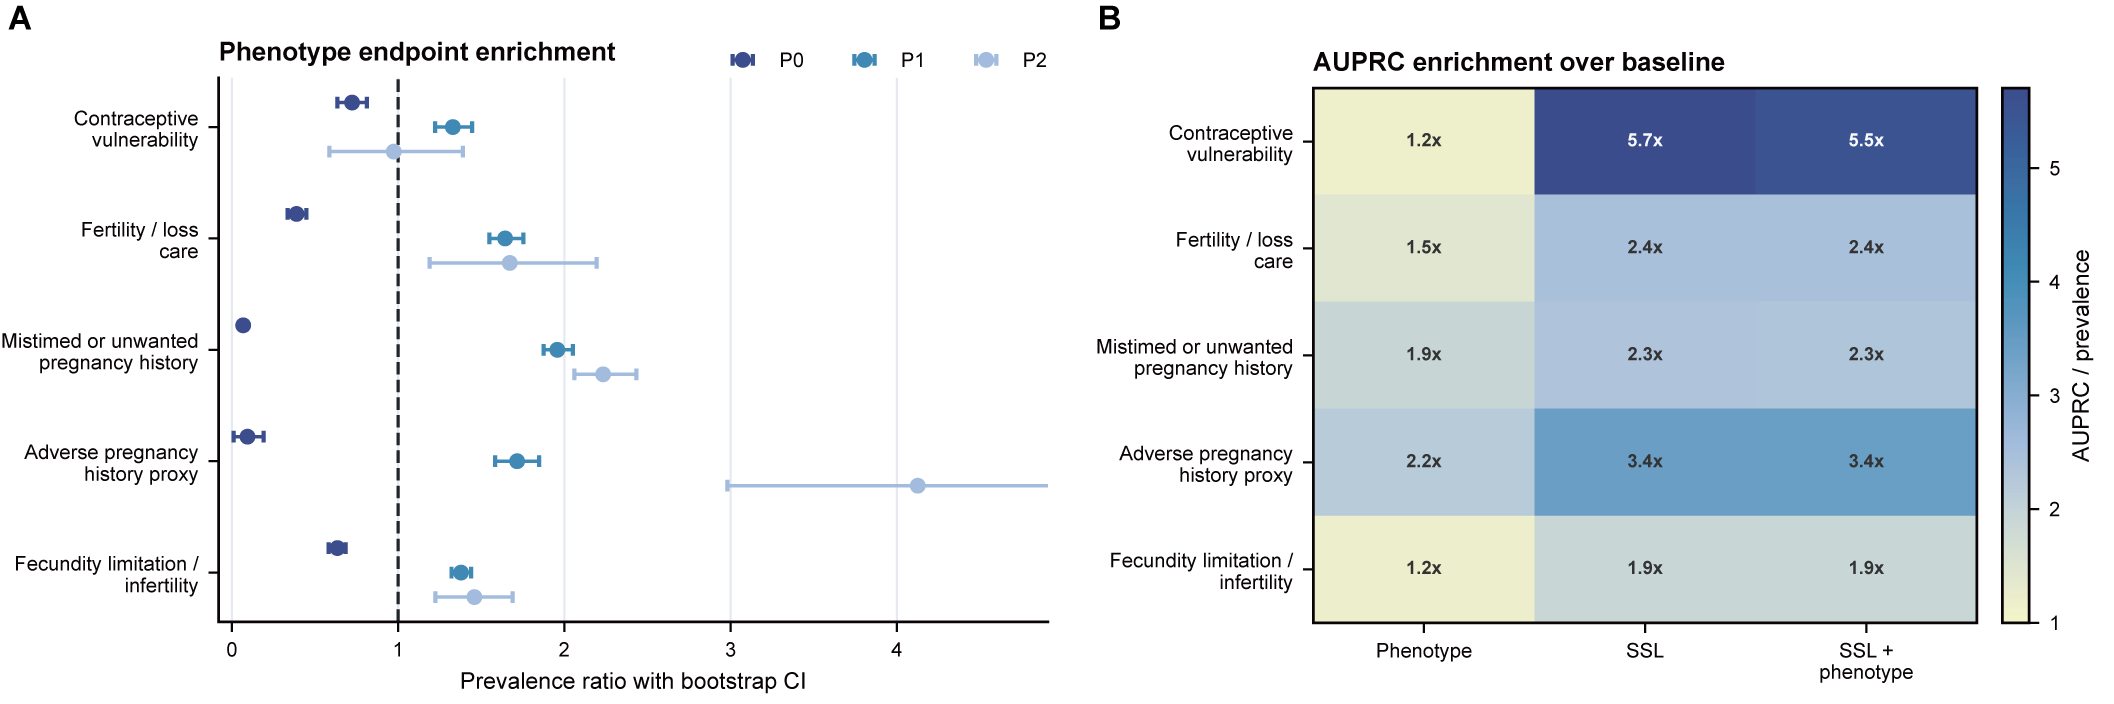
\includegraphics[width=\textwidth]{figures/FIG5.png}
\caption{Endpoint enrichment and secondary supervised endpoint-enrichment summaries. (A) Full analytic-cohort survey-weighted prevalence ratios by phenotype in the 2022--2023 within-NSFG temporal-validation cohort with stratified cluster bootstrap confidence intervals; pregnancy-history endpoints are interpreted primarily using the ever-pregnant estimates in Table 4 and Supplementary Table 8. The dashed vertical line indicates no enrichment. (B) AUPRC enrichment over baseline prevalence for phenotype-only, SSL-embedding, and SSL-plus-phenotype summaries.}
\label{fig:enrichment}
\end{figure}

\subsection{Robustness and sensitivity analyses}

Age-range sensitivity analyses preserved the main enrichment direction after including 45--49-year-old respondents from the 2022--2023 public-use release. Reassignment quality for the 15--44 subset was checked only as a technical reproducibility control (ARI 1.00) and was not treated as independent robustness evidence. The highest phenotype PR for adverse pregnancy-history proxy attenuated from 4.11 in ages 15--44 to 3.25 in ages 15--49, and the highest PR for mistimed or unwanted pregnancy history changed from 2.23 to 1.98; all prespecified endpoints retained the same enrichment direction in the expanded age range. Because 45--49-year-old respondents were assigned by a model developed in ages 15--44, this analysis was interpreted as a sensitivity stress test rather than a fully validated expanded-age model. Supplementary Table 3 and Supplementary Figure S1 report the age-range sensitivity analysis.

The adjusted enrichment models are reported in Supplementary Table 4. Covariate-adjusted enrichment models showed that some, but not all, unadjusted phenotype enrichments persisted after accounting for age, race/ethnicity, education, poverty, insurance, and parity. P2 remained enriched for adverse pregnancy-history proxy after adjustment (adjusted OR 2.05, 95\% CI 1.20--3.57). P1 remained enriched for contraceptive vulnerability (adjusted OR 1.84, 95\% CI 1.39--2.41), fertility-service or pregnancy-loss help (adjusted OR 2.50, 95\% CI 1.92--3.56), and mistimed or unwanted pregnancy history (adjusted OR 9.58, 95\% CI 7.69--12.81). The large P1 adjusted OR for mistimed or unwanted pregnancy history and the near-null or protective estimates for P0 should be read as exposure-structure signals from pregnancy-record definability, not as independent phenotype effects. By contrast, the unadjusted P2 fecundity limitation/infertility enrichment was not robust after adjustment (adjusted OR 0.99, 95\% CI 0.67--1.33). These adjusted models reconcile the unadjusted PRs with covariate-conditioned descriptive associations and do not imply causal phenotype effects.

Baseline-method, leakage, subgroup, ever-pregnant, simple-strata, raw-feature supervised, and seed-sensitivity outputs are reported in Supplementary Table 5 through Supplementary Table 11; the corresponding method-sensitivity and subgroup displays are reported in Supplementary Figures S2 and S3. Specifically, leakage sensitivity is reported in Supplementary Table 6, subgroup robustness in Supplementary Table 7, the ever-pregnant stratum in Supplementary Table 8, and simple age/parity baselines in Supplementary Table 9. Baseline method comparisons supported the stability, rather than universal enrichment superiority, of the SSL phenotype representation. SSL embedding plus k-means had development bootstrap ARI 0.953 and a minimum temporal-validation cluster proportion of 4.9\%. This supplementary baseline clusters the SSL embedding directly; the primary phenotype-selection workflow first projects embeddings to principal components and therefore has the development bootstrap ARI reported in Figure 3 and Supplementary Table 1. Raw matrix PCA plus k-means produced a much smaller minimum cluster proportion (0.1\%), indicating that some high enrichment values from raw PCA reflected unstable tiny clusters. Selected-variable Bernoulli LCA had development bootstrap ARI 0.904 but lower average endpoint-enrichment summaries than SSL. In leakage sensitivity, the full-domain encoder did not uniformly exceed the endpoint-excluded encoder; for adverse pregnancy-history proxy, the maximum PR was 4.13 for the primary endpoint-excluded encoder versus 2.01 for the full-domain encoder.

The simple stratification baseline confirmed that pregnancy-history endpoint enrichment was partly recoverable from age and pregnancy exposure alone. In the ever-pregnant stratum, the top age-by-parity group had PR 1.46 for adverse pregnancy-history proxy, compared with P2 PR 2.16; for mistimed or unwanted pregnancy history, the corresponding PRs were 1.21 and 1.17. Full-cohort age-by-parity enrichment for adverse pregnancy-history proxy was also high (PR 2.91), reinforcing that full-cohort pregnancy-history results should not be read as independent phenotype effects. Fixed-k encoder initialization sensitivity showed that an alternative 30-epoch seed had lower agreement with the primary temporal-validation assignment (ARI 0.43) but retained ever-pregnant adverse pregnancy-history enrichment above null (maximum PR 1.68). Subgroup summaries showed enrichment patterns across demographic and reproductive-history strata, but extreme subgroup values were treated as unstable when they arose from small event counts.

\section{Discussion}

This temporal survey analysis shows that masked tabular SSL can summarize NSFG female respondent and pregnancy files into interpretable reproductive life-course profiles. The main informatics contribution is not a new single-endpoint risk score or clinical prediction model, but a reproducible workflow for learning survey-based respondent representations, translating them into profile-based phenotypes, and auditing whether endpoint enrichment survives leakage controls, raw-feature baselines, and simple exposure-structure baselines. This framing is intended for population reproductive-health surveillance and hypothesis generation, not for clinical triage or individual counseling.

The three-phenotype solution separated a younger low-pregnancy-exposure group, a main pregnancy-exposed group, and a small higher-burden pregnancy-history group. This structure is consistent with the descriptive reproductive-health logic that survey-measured reproductive needs emerge from combinations of age, pregnancy history, partnership and contraceptive context, fertility services, and fecundity status rather than from any single endpoint variable. The phenotype interpretation remained profile-based, avoiding naming clusters solely by their validation endpoints.

For reproductive-health surveillance, the practical use case is cohort-level stratification rather than individual risk prediction. Public-health analysts could use similar profiles to monitor whether contraceptive vulnerability, fertility-service needs, fecundity limitation, or adverse pregnancy-history proxies concentrate within stable life-course strata across survey cycles, demographic groups, or policy-relevant access categories. The profiles can also help prioritize descriptive subgroup audits and generate hypotheses for more detailed clinical or registry studies. They should not be used to assign individual diagnoses, guide bedside management, or replace domain-specific NSFG surveillance reports.

The strongest full-cohort unadjusted enrichment occurred for pregnancy-history endpoints in the small P2 phenotype. Because pregnancy-record availability, parity, and pregnancy-history summaries are themselves part of the life-course structure, these findings can be partly exposure-driven. The age-by-parity and age-by-ever-pregnant baselines confirmed this concern: simple strata reproduced a substantial portion of pregnancy-history enrichment, especially in the full analytic cohort. For this reason, the ever-pregnant stratum was used as the primary interpretive analysis for pregnancy-history endpoints: it reduced mechanical enrichment from pregnancy exposure and showed that adverse pregnancy-history enrichment persisted but attenuated. Adjusted models further showed that some unadjusted signals, especially fecundity limitation/infertility in P2, were not robust after age, sociodemographic, insurance, and parity adjustment. These patterns support descriptive phenotype enrichment rather than causal inference or independent clinical prediction.

The raw-feature supervised comparison provides a complementary view of representation utility. SSL embeddings outperformed the raw 48 primary inputs in the prespecified L2-logistic AUPRC summaries in this temporal split, including the ever-pregnant pregnancy-history analyses. However, the supervised gains should be interpreted cautiously because the models were not calibrated clinical risk tools, the endpoints are public-use survey constructs, and the embedding did not make phenotype labels consistently additive. The practical value of the SSL layer is therefore compression, harmonized cross-domain representation, and sensitivity-audited endpoint enrichment rather than a claim that deep learning is necessary for every NSFG endpoint.

The study differs from prior NSFG reports and analyses that focus on specific domains such as contraceptive status, fertility services, birth expectations, adolescent pregnancy intention classes, IUD use across life stages, or contraceptive non-use \cite{cdc_db539,cdc_db542,cdc_db560,adolescent_lca,iud_lifecourse,contraceptive_nonuse}. Those analyses remain essential for domain-specific surveillance and policy; our analysis adds a multivariable representation-learning layer that can summarize cross-domain reproductive life-course heterogeneity in public-use survey data.

Several limitations are important. First, NSFG public-use data are self-reported and do not contain hospital-verified clinical outcomes. Endpoint definitions therefore rely on public-use survey recodes and should be interpreted as reproductive-health proxies. Second, validation was temporal within the NSFG public-use survey series rather than external validation in an independent survey, hospital EHR, or registry. The 2022--2023 release also used a redesigned continuous, multimode protocol with an online component, so differences between 2017--2019 and 2022--2023 may reflect both temporal change and survey-mode or instrument change. Third, the higher-burden P2 phenotype was small in the development and temporal-validation cohorts; this supports interpretability but limits precision, especially for subgroup estimates with few events. Fourth, endpoint leakage was reduced by direct-variable exclusion and was examined with a full-domain sensitivity encoder, but public-use survey variables are correlated, and pregnancy counts, parity, and pregnancy-history summaries can serve as indirect proxies for pregnancy-history endpoints. The ever-pregnant stratum and simple-strata baselines address but do not eliminate this concern. Fifth, adjusted enrichment and subgroup analyses reduce concern that phenotypes merely restate age or parity gradients, but they remain descriptive robustness checks and do not identify causal mechanisms. Sixth, the SSL objective and cluster-selection procedure did not optimize a design-based survey likelihood; survey design variables and weights were used for descriptive profiles and enrichment intervals rather than for representation learning itself. Seventh, fixed-k seed sensitivity suggested that transferred phenotype assignments were moderately initialization-sensitive, even though endpoint enrichment direction persisted for adverse pregnancy-history proxy; therefore, the exact cluster boundaries require independent replication. Finally, the compact encoder was designed for reproducible CPU-feasible public-data analysis and should not be framed as a large foundation model.

\section{Conclusions}

A leakage-controlled masked tabular SSL workflow identified interpretable reproductive life-course profiles in public-use NSFG data and demonstrated descriptive within-NSFG endpoint enrichment for multiple reproductive-health survey endpoints. Simple-strata and raw-feature comparisons showed both the value and limits of the representation: SSL embeddings improved secondary AUPRC summaries relative to raw 48 inputs in this split, but pregnancy-history phenotype enrichment remained partly recoverable from age and pregnancy-exposure strata. The approach provides a reproducible framework for population-level reproductive-health phenotyping, while future work should pursue independent survey or registry replication, survey-design-aware uncertainty intervals, broader seed-sensitivity testing, and cautious applied interpretation.

\backmatter

\section*{Declarations}

\bmhead{Availability of data and materials}

The raw data analyzed in this study are publicly available from CDC/NCHS NSFG public-use data portals, including the 2022--2023 public-use files and 2011--2019 public-use releases. Raw individual-level public-use records are not redistributed in this manuscript package. Processed source-data tables used for figures and manuscript tables are included in the \texttt{source\_data} directory and archived with the reproducibility package at Zenodo: \url{https://doi.org/10.5281/zenodo.20692052}. Public-use data access URLs and parsing notes are documented in the project README and processing scripts.

\bmhead{Code availability}

Analysis scripts, split definitions, source-data tables, model metadata, and figure assets are available at GitHub (\url{https://github.com/Luciky-Leo/nsfg-reproductive-lifecourse-ssl}) and Zenodo (\url{https://doi.org/10.5281/zenodo.20692052}). Raw NSFG individual-level public-use records are not redistributed; the scripts point to CDC/NCHS public-use data portals and document the processing workflow. Project code is released under the MIT License, and citation metadata are provided in \texttt{CITATION.cff}. The submitted package includes the feature-audit files needed to identify primary encoder inputs, candidate retained variables, excluded sparse variables, and endpoint-direct exclusion rules.

\bmhead{Ethics approval and consent to participate}

This study used de-identified public-use NSFG data released by CDC/NCHS. No new human-subject data were collected, and the analysis involved no direct participant contact or identifiable private information; therefore, separate informed consent and institutional review board approval were not required for this secondary public-use analysis.

\bmhead{Consent for publication}

Not applicable.

\bmhead{Competing interests}

The authors declare no competing interests.

\bmhead{Funding}

No external funding was received for this study.

\bmhead{Authors' contributions}

Feifan Lu, Fengshang Yan, and Qianqian Yang contributed equally to this work. Feifan Lu contributed to study conceptualization, public-data curation, formal analysis, figure and table generation, and manuscript drafting. Fengshang Yan and Qianqian Yang contributed to data verification, result interpretation, manuscript review, and revision. Jiuqiong Yan contributed to clinical interpretation, supervision, manuscript review, and revision. Rui Guan supervised the study, provided senior oversight, reviewed and edited the manuscript, and approved the final version. All authors read and approved the final manuscript.

\bmhead{Use of artificial intelligence assisted tools}

The authors used AI-assisted tools for language editing, formatting support, code-drafting support, and internal consistency checks during manuscript preparation. All analyses, interpretations, final text, figures, and submitted materials were reviewed and approved by the authors, who take full responsibility for the content.

\bmhead{Supplementary information}
Supplementary tables and figures are provided in the separate file \texttt{supplementary\_information.pdf}.

\begin{thebibliography}{99}
\bibitem{finer_zolna_unintended} Finer LB, Zolna MR. Declines in unintended pregnancy in the United States, 2008--2011. N Engl J Med. 2016;374(9):843--852. doi:10.1056/NEJMsa1506575.
\bibitem{contraceptive_failure} Sundaram A, Vaughan B, Kost K, Bankole A, Finer L, Singh S, Trussell J. Contraceptive failure in the United States: estimates from the 2006--2010 National Survey of Family Growth. Perspect Sex Reprod Health. 2017;49(1):7--16. doi:10.1363/psrh.12017.
\bibitem{infertility_impaired} Chandra A, Copen CE, Stephen EH. Infertility and impaired fecundity in the United States, 1982--2010: data from the National Survey of Family Growth. Natl Health Stat Report. 2013;(67):1--18.
\bibitem{infertility_service} Chandra A, Copen CE, Stephen EH. Infertility service use in the United States: data from the National Survey of Family Growth, 1982--2010. Natl Health Stat Report. 2014;(73):1--21.
\bibitem{contraceptive_nonuse} Frederiksen BN, Ahrens K. Understanding the extent of contraceptive non-use among women at risk of unintended pregnancy, National Survey of Family Growth 2011--2017. Contraception: X. 2020;2:100033. doi:10.1016/j.conx.2020.100033.
\bibitem{cdc_nsfg_puf} National Center for Health Statistics. National Survey of Family Growth: 2022--2023 public-use data files, codebooks, and documentation. https://www.cdc.gov/nchs/nsfg/nsfg-2022-2023-puf.htm.
\bibitem{cdc_nsfg_combined} National Center for Health Statistics. 2011--2019 combined files: selected data and documentation. \url{https://www.cdc.gov/nchs/nsfg/nsfg_2011_2019_combined_files.htm}.
\bibitem{cdc_db539} National Center for Health Statistics. Current contraceptive status among females ages 15--49: United States, 2022--2023. NCHS Data Brief No. 539. 2025. https://www.cdc.gov/nchs/products/databriefs/db539.htm.
\bibitem{cdc_db542} National Center for Health Statistics. Use of fertility services in the United States, 2022--2023. NCHS Data Brief No. 542. 2025. https://www.cdc.gov/nchs/products/databriefs/db542.htm.
\bibitem{cdc_db560} Martinez GM. Birth expectations of women ages 20--49: United States, 2022--2023. NCHS Data Brief No. 560. 2026. https://www.cdc.gov/nchs/products/databriefs/db560.htm.
\bibitem{vime} Yoon J, Zhang Y, Jordon J, van der Schaar M. VIME: extending the success of self- and semi-supervised learning to tabular domain. Advances in Neural Information Processing Systems. 2020;33:11033--11043.
\bibitem{tabtransformer} Huang X, Khetan A, Cvitkovic M, Karnin Z. TabTransformer: tabular data modeling using contextual embeddings. arXiv:2012.06678. 2020. https://arxiv.org/abs/2012.06678.
\bibitem{saint} Somepalli G, Goldblum M, Schwarzschild A, Bruss CB, Goldstein T. SAINT: improved neural networks for tabular data via row attention and contrastive pre-training. arXiv:2106.01342. 2021. https://arxiv.org/abs/2106.01342.
\bibitem{scarf} Bahri D, Jiang H, Tay Y, Metzler D. SCARF: self-supervised contrastive learning using random feature corruption. arXiv:2106.15147. 2021. https://arxiv.org/abs/2106.15147.
\bibitem{tabular_tree} Grinsztajn L, Oyallon E, Varoquaux G. Why do tree-based models still outperform deep learning on tabular data? Advances in Neural Information Processing Systems. 2022;35:507--520.
\bibitem{lumley_survey} Lumley T. Analysis of complex survey samples. J Stat Softw. 2004;9(8):1--19. doi:10.18637/jss.v009.i08.
\bibitem{strobe} von Elm E, Altman DG, Egger M, Pocock SJ, Gotzsche PC, Vandenbroucke JP; STROBE Initiative. The Strengthening the Reporting of Observational Studies in Epidemiology (STROBE) Statement: guidelines for reporting observational studies. PLoS Med. 2007;4(10):e296. doi:10.1371/journal.pmed.0040296.
\bibitem{tripod_ai} Collins GS, Moons KGM, Dhiman P, Riley RD, Beam AL, Van Calster B, et al. TRIPOD+AI statement: updated guidance for reporting clinical prediction models that use regression or machine learning methods. BMJ. 2024;385:e078378. doi:10.1136/bmj-2023-078378.
\bibitem{adolescent_lca} Offiong A, Powell TW, Dangerfield DT, Gemmill A, Marcell AV. A latent class analysis: identifying pregnancy intention classes among U.S. adolescents. J Adolesc Health. 2022;71(4):466--473. doi:10.1016/j.jadohealth.2022.04.019.
\bibitem{iud_lifecourse} Kramer RD, Higgins JA, Godecker AL, Ehrenthal DB. Reconsidering (in)equality in the use of IUDs in the United States: a closer look across the reproductive life course. Demographic Research. 2020;43:1049--1066. doi:10.4054/DemRes.2020.43.35.
\end{thebibliography}

\end{document}
